\section{Data Sources}
\label{sec:data}

The study retrospectively included 3 different datasets with a total of 3025 DAT-SPECT images.
The primary dataset (`development dataset') was used for both training and testing the models associated with the respective method, 
whereas the other two datasets, the \textit{PPMI} dataset and the \textit{MPH} dataset were used for testing only, not for training.

\subsection{Development dataset}
\label{subsec:spect_dataset}

The development dataset consisted of 1740 consecutive DAT-SPECT scans obtained from clinical routine at 
the Department of Nuclear Medicine, University Medical Center Hamburg-Eppendorf~\citep{Schiebler2023}.
In brief, DAT-SPECT with [$^{123}$I]FP-CIT had been performed according to common procedures guidelines~\citep{Darcourt2010-ar, Djang2012-ow} 
with different double-head cameras equipped with low-energy-high-resolution or fan-beam collimators. 
The projection data were reconstructed using the iterative ordered-subsets-expectation-maximization~\citep{Hudson1994} 
with attenuation and simulation-based scatter correction 
as well as collimator-detector response modeling as implemented in the Hybrid Recon-Neurology tool 
of the Hermes SMART workstation v1.6 (Hermes Medical Solutions, Stockholm, Sweden)~\citep{Diemling2021-mg, Sohlberg2012-ep, HybridRecon, Kangasmaa2016-aw}.
All parameter settings were as recommended by Hermes~\citep{Diemling2021-mg} for the EANM / EANM Research Ltd (EARL) ENC-DAT project (European Normal Control Database of DaTSCAN)~\citep{Tossici-Bolt2011-cx, Dickson2010-fm, Varrone2013-it, Tossici-Bolt2017-xj, Dickson2012-hk}.
More precisely, ordered-subsets-expectation-maximization was performed with 5 iterations and 15/16 subsets for 120/128 views. 
For noise suppression, reconstructed images were postfiltered by convolution with a 3-dimensional Gaussian kernel of 7 mm full-width-at-half-maximum. 

The ground-truth label, indicating either `normal' or `Parkinson-typical' reduction (`reduced') of the striatal signal, 
was obtained by visual assessment of the DAT-SPECT images by three independent readers~\citep{Schiebler2023}. 
The readers achieved inter-reader consensus on the `normal' label in 855 cases ($49.1\%$)
and on the `reduced' label in 802 cases ($46.1\%$).
The inter-reader consensus on the label could not be achieved for 83 cases ($4.8\%$).
The dataset comprised about $43.5\%$ female cases and $56.5\%$ male cases.
In the dataset, the average age among cases was $66.7$ with a standard deviation of $11.6$ years.
The development dataset was utilized for both training and testing the classification models. 

\subsection{Independent testing datasets}
\label{subsec:external_dataset}

The second dataset comprised 645 DAT-SPECT with [$^{123}$I]FP-CIT from the Parkinson's Progression Markers Initiative (PPMI) 
(www.ppmi-info.org/data)~\citep{Parkinson_Progression_Marker_Initiative2011-px}.
The external dataset included 438 patients with Parkinson's disease and 207 healthy controls as described in~\cite{Wenzel2019}.
The mean age among cases was $61.2$ with a standard deviation of $10.2$ years, 
and the dataset comprised $35.2\%$ female cases.
Details of the PPMI DAT-SPECT protocol are given at http://www.ppmi-info.org/study-design/research-documents-and-sops/ ~\citep{Parkinson_Progression_Marker_Initiative2011-px}. 
Raw projection data has been transferred to the PPMI imaging core lab for central image reconstruction using an iterative (HOSEM) algorithm on a HERMES workstation. 
The clinical diagnosis was used as ground-truth label (Parkinson's disease = ``reduced", healthy control = ``normal"). 
The external dataset showed lower spatial resolution than the development dataset (lower striatum-to-background contrast).

The third dataset (`MPH dataset') comprised 640 consecutive DAT-SPECT with [$^{123}$I]FP-CIT from clinical routine at UKE 
that had been acquired with a triple-head camera equipped with brain-specific multiple pinhole (MPH) collimators. 
Multiple pinhole SPECT concurrently improves count sensitivity and spatial resolution compared to SPECT with parallel-hole 
and fan-beam collimators~\citep{Mathies2022-yi, Tecklenburg2020-xr}.
The projection data were reconstructed with the Monte Carlo photon simulation engine 
and iterative one-step-late maximum-a-posteriori expectation-maximization implemented 
in the camera software (24 iterations, 2 subsets)~\citep{Tecklenburg2020-xr, Magdics2010}.
Neither attenuation nor scatter correction was applied to the SPECT images.
The ground-truth label (`normal' or `reduced') was obtained by the visual interpretation of an experienced reader 
(about 20 years of experience in clinical DAT-SPECT reading, $\geq$3,000 cases).
All SPECT images were interpreted twice (with different randomization) by the same reader. 
The delay between the reading sessions was 14 days. 
Cases with discrepant interpretations between the two reading sessions were read a third time by the same reader 
to obtain an intra-reader consensus as the ground-truth label. 
Thereby 327 cases ($51.09\%$) were labeled as `reduced'  and 313 cases ($48.91\%$) were labeled as `normal'.
The average age among cases was $67.2$ with a standard deviation of $11.4$ years.
In contrast to the development dataset, the internal test dataset exhibited a better spatial resolution, 
leading to higher contrast between the striatum and background, along with reduced statistical noise.
The MPH dataset has not been described in previous works.

Figure~\ref{fig:datasets_samples} illustrates example DVR slabs for one `normal' case and three `reduced' cases obtained
from the development dataset, the PPMI dataset, and the MPH dataset.

\begin{figure}[t]
    \centering
    \colorbox{black}{%
     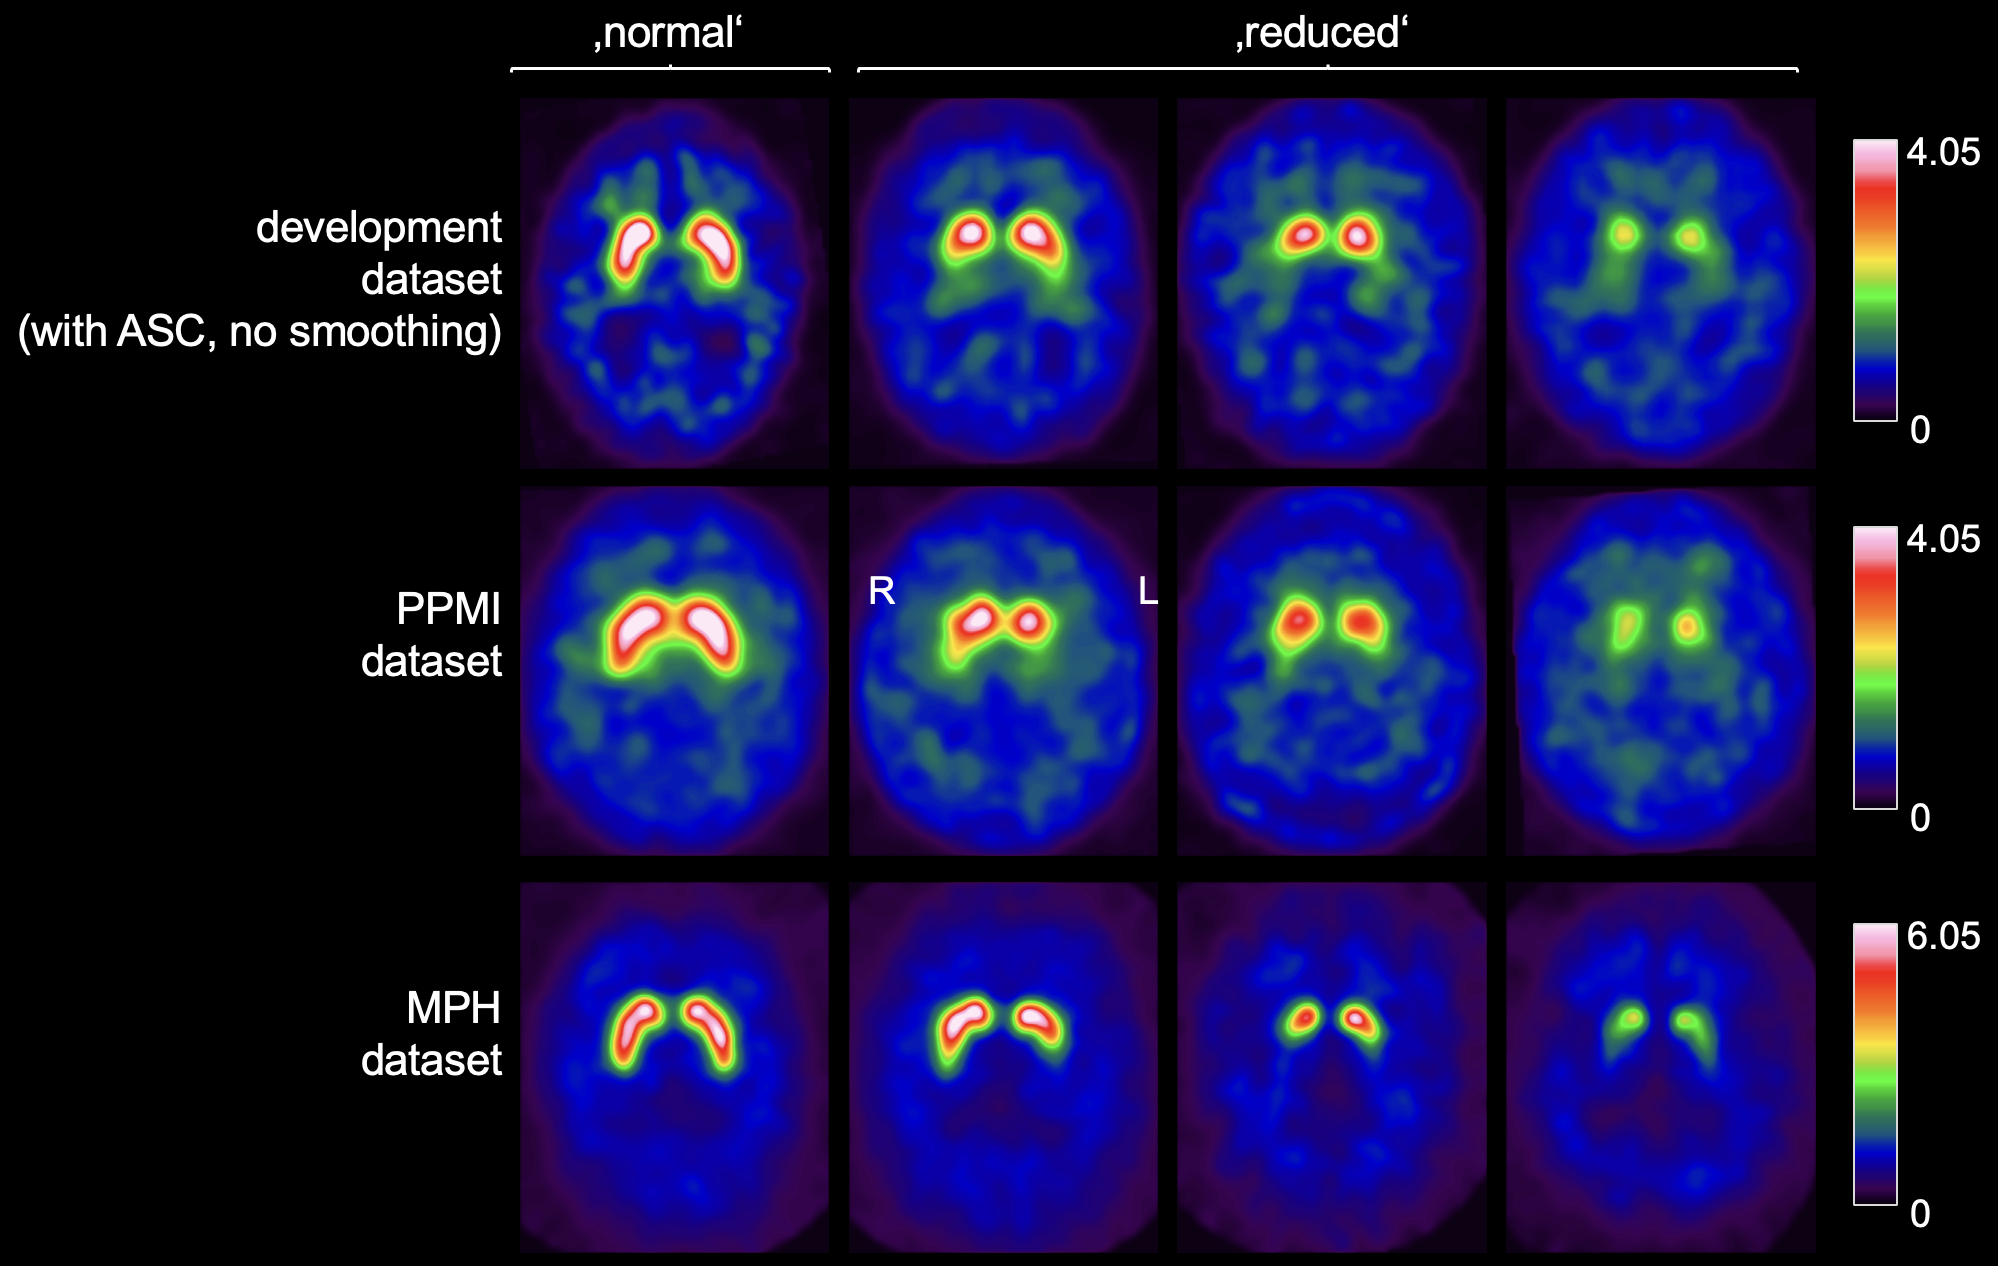
\includegraphics[width=0.95\textwidth]{content/figures/datasets_samples.png}%
     }
    \caption{DVR slabs for one healthy control (`normal') case 
    and three cases with reduced availability of DAT in the striatum (`reduced')
    from the development dataset, the PPMI dataset, and the MPH dataset.
    For the cases from the development dataset, attenuation and scatter correction (ASC) were applied, 
    and no smoothing was performed.} 
    \label{fig:datasets_samples}
\end{figure}
